%\documentclass[12pt]{article}
%\usepackage{graphicx,amssymb,epsf}

%\begin{document}

Double Deep Virtual Compton Scattering (DDVCS), in the context
of Jefferson Lab, stands for the reaction:
$ep\to ep\gamma^*\hookrightarrow \ell^+\ell^-$, i.e. the exclusive
electroproduction on the protonon of a 
timelike photon which decays into a pair of leptons $\ell$
(electrons or muons in the present case). 

It is a generalization of Deep Virtual Compton Scattering (DVCS):
$ep\to ep\gamma$ (i.e. with a real photon in the final state)
and Timelike Compton Scattering (TCS): 
$\gamma p\to p\gamma^*\hookrightarrow \ell^+\ell^-$
(i.e. with a real photon in the initial state). For virtualities 
of the virtual photons large enough ($Q^2=(e-e')^2$ for DVCS
or $Q'^2=(\ell^++\ell^-)^2$ for TCS) and small nucleon
momentum transfer $t=(p-p')^2$, it has been 
shown that these reactions are probing the
internal quark and gluon structure of the nucleon via
the formalism of the Generalized Parton Distributions (GPDs).
See Refs.~\cite{goeke,revdiehl,revrady,rpp} for reviews on the subject
of GPDs and DVCS and Refs.~\cite{Berger:2001xd,Goritschnig,Boer:2015hma}
for studies of TCS. See Fig.\ref{fig:diags} for a sketch of the
DVCS, TCS and DDVCS processes. These so-called ``handbag" diagrams
illustrate the QCD factorization theorem behind the formalism
of GPDs: in the Bjorken regime, the processes are the (convolution) product
of a hard scattering part exactly calculable in QED, i.e. the
elementary photon-quark scattering $\gamma q\to\gamma q$, and
and soft non-perturbative QCD matrix elements, called the GPDs
for their momentum space representation.

\begin{figure}[htbp]
\begin{center}
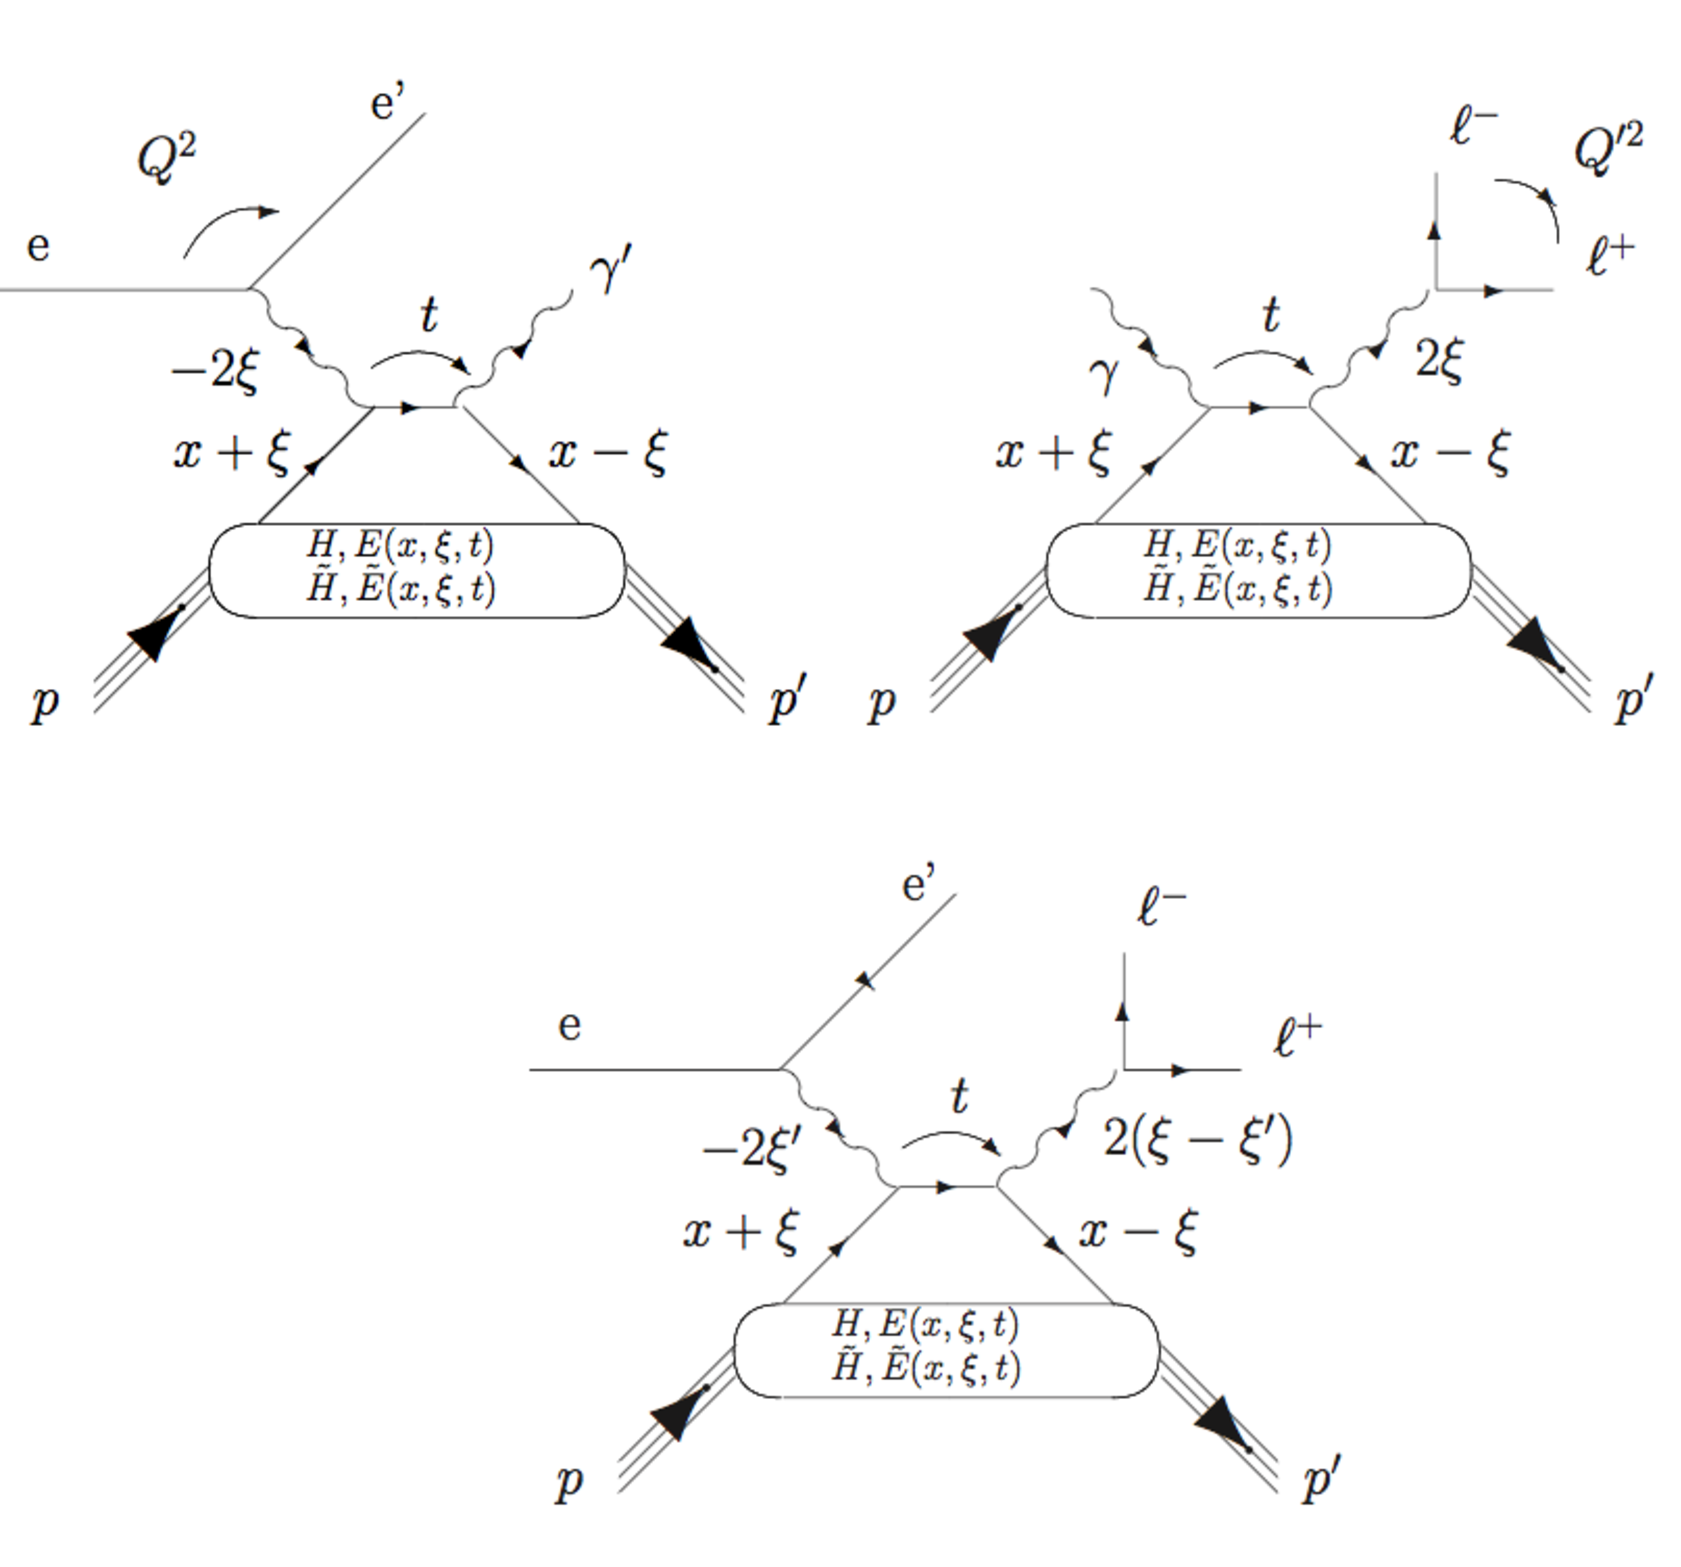
\includegraphics[width=1\textwidth]{3proc.pdf}
\end{center}
\caption{Top left: DVCS handbag diagram. Top right: TCS handbag diagram.
Bottom: DDVCS handbag diagram. Only ``direct" diagrams are shown. There are
also ``crossed" diagrams. In a frame where the nucleon
moves at the speed of light along a certain direction, the longitudinal 
momentum fractions of the particles are also indicated.}
\label{fig:diags}
\end{figure}

There are, at leading twist QCD, four GPDs, called
$H, \tilde H, E, \tilde E$ which reflect the four independent
quark-nucleon helicity-spin transitions between the initial
and final states. They depend upon three variables~: 
$x$, $\xi$ and $t$. As illustrated in Fig.~\ref{fig:diags},
$x+\xi$ is the {\it longitudinal} momentum fraction carried by 
the initial quark struck by the spacelike virtual photon and $x-\xi$ is 
{\it longitudinal} momentum fraction carried by the final quark going 
back in the nucleon after radiating a photon. In Ji's notation~\cite{Ji:1996nm},
the variable varies $x$ between $-1$ and $1$ while the variable $\xi$ 
varies between $0$ and $1$ (due to time reversal invariance, the range of $\xi$ 
can be reduced to this range). One way to interpret the GPDs is therefore as
the probability amplitude of finding a quark (if $|x| > \xi$, or an antiquark 
if $x<-\xi$) in the nucleon with a longitudinal momentum fraction $x+\xi$
and of putting it back into the nucleon with a longitudinal momentum
fraction $x-\xi$ plus some transverse momentum ``kick", which is
represented by $t$. One notes the interesting region $ -\xi < x < \xi$ 
where one ``leg" in Fig.~\ref{fig:diags} 
has a positive momentum fraction (a quark) while the other one has a negative one
(an antiquark). In this region, GPDs behave like a meson distribution amplitude
and can be interpreted as the probability amplitude of finding 
a quark-antiquark pair in the nucleon. 
At $\xi=0$, $t$ can be interpreted as the conjugate variable of the
{\it transverse} impact parameter $b_\perp$ and GPDs describe then the probability 
amplitude of finding in a nucleon a parton with a {\it longitudinal} momentum 
fraction $x$ at a given {\it transverse} distance $b_\perp$ from the
center of the nucleon.

\begin{figure}[htbp]
%\begin{minipage}[t]{76mm}
\begin{center}
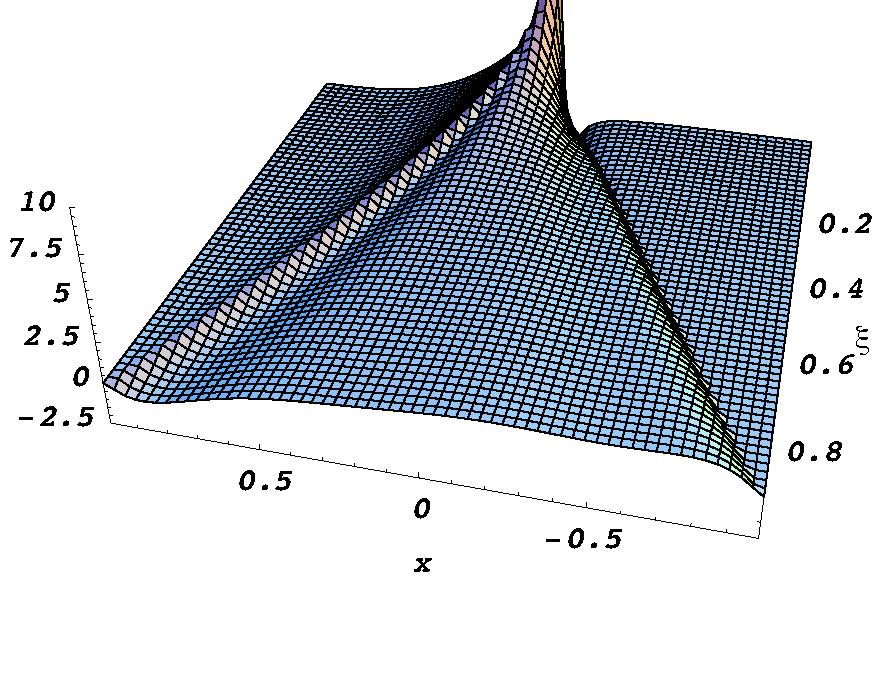
\includegraphics[width=0.7\textwidth]{gpdxxi.pdf}
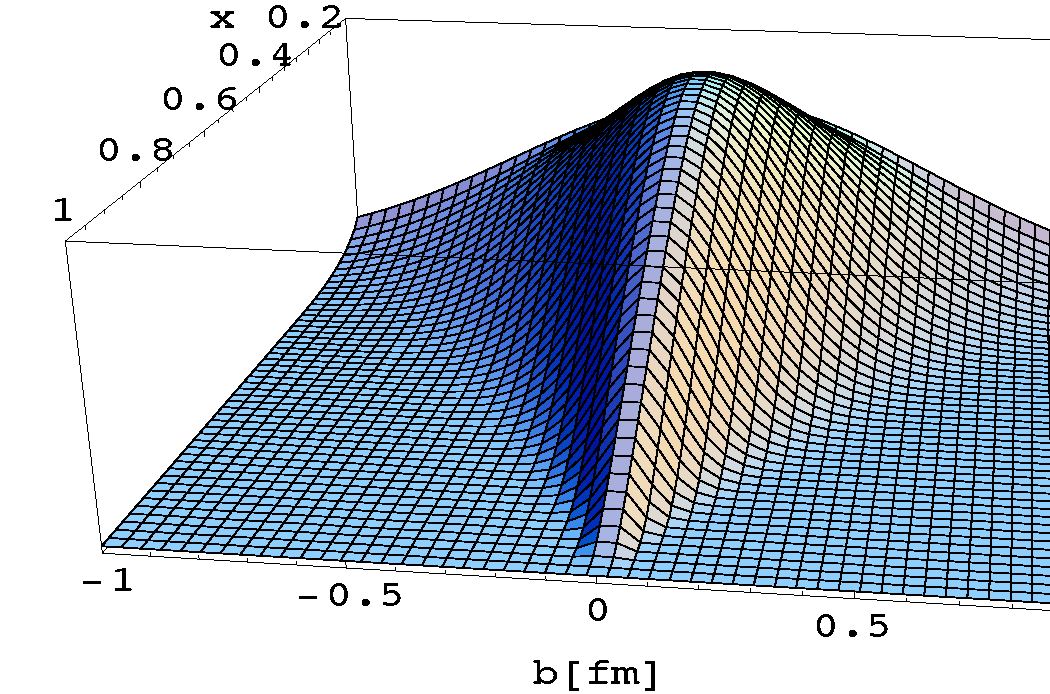
\includegraphics[width=0.7\textwidth]{gpdb_h_u_new.pdf}
%\end{minipage}
%\vspace{-2cm}
\caption{Top: the GPD $H^u(x,\xi,t)$ as a function of the 
{\it longitudinal} momentum fraction $x$ and the {\it longitudinal} 
momentum transfer $\xi$ at $t=0$ according to the VGG model.
One recognizes for $\xi$=0 the typical shape of a parton distribution (with 
the sea quarks rising as $x$ goes to 0, the negative $x$ part being interpreted 
as the antiquark contribution) and as $\xi$ increases the (asymptotic) shape of
a distribution amplitude. Bottom: the GPD $H^u(x,\xi,t)$ as 
a function of the {\it longitudinal} momentum fraction $x$ and 
the {\it transverse} impact parameter $b_\perp$ (the conjugate variable of $t$)
at $\xi=0$ according to the VGG model}
\label{fig:gpdxxi-bperp}
\end{center}
\end{figure}

Fig.~\ref{fig:gpdxxi-bperp} shows, according to one patricular 
GPD model (VGG~\cite{marcprl2,goeke}),
how the ($x$,$\xi$) and the ($x$,$b_\perp$) correlations could look like.
It shows the richness and novelty of the GPDs: information on
$q{\bar q}$ configurations in the nucleon, correlations between quarks 
(or antiquarks) of different momenta, correlations between longitudinal
momentum and trsanverse position of partons (nucleon ``tomography").

We have just seen a crucial issue in the GPD formalism is that the GPDs 
depend on three variables~: $x$, $\xi$ and $t$, but only two of these 
three variables are accessible experimentally, $\xi$ and $t$.
In DVCS, $\xi$ is approximated as $\xi=\frac{x_B}{2-x_B}$, fully
defined by detecting the scattered lepton, and in TCS, $\xi$
is approximateded as $\xi=\frac{Q'^2}{2s-Q'^2}$, fully defined by 
detecting the final leptons.% (all at given beam energies).

The squared momentum transfer $t$ is defined both in DVCS and in TCS by 
detecting either the recoil proton or the outgoing photon.
The variable $x$ is however integrated over in both the DVCS and TCS
amplitudes, due to the loop in the ``handbag" diagrams (see Fig.~\ref{fig:diags}).
Precisely, the DVCS amplitude is proportional to:
\begin{eqnarray}
\int_{-1}^{+1}d x {{H(x,\xi,t)} \over {x - \xi + i \epsilon}}+...
\end{eqnarray}
(where the ellipsis stand for similar terms in $E$, $\tilde{H}$
and $\tilde{E}$). 
The ${1} \over {x - \xi + i \epsilon}$ term is the propagator of the quark 
between the incoming virtual photon and the outgoing photon.
The previous expression can be decomposed into a real and an imaginary parts:
\begin{eqnarray}
PV(\int_{-1}^{+1}d x {H(x,\xi,t) \over {x - \xi}})-i\pi H(\xi,\xi,t)
\end{eqnarray}
This means that the maximum information that can be extracted from the experimental 
data at a given ($\xi,t$) point is $H(\pm\xi,\xi,t)$, when measuring an observable
particularly sensitive to the imaginary part of the DVCS amplitude (such as single beam 
or target spin asymmetries), and $\int_{-1}^{+1}d x {H(\mp x,\xi,t) 
\over {x \pm \xi}}$, when measuring an observable particularly
sensitive to the real part of the DVCS amplitude (such as unpolarized
cross sections or double-spin beam/target spin asymmetries).

Experimentally, DVCS is accessed by measuring the reaction $ep\to e p\gamma$
and TCS by measuring the reaction $\gamma p\to p \ell^+\ell^-$. However,
DVCS and TCS are not the only processes leading to these final states. There
are also the so-called Bethe-Heitler (BH) processes. In the $ep\to e p\gamma$ reaction,
the BH produces a final state photon which is radiated either
from the incoming or the scattered electron and in the $\gamma p\to p \ell^+\ell^-$,
the final lepton pair originates from the photon beam (see Fig.~\ref{fig:allbh}). 
In both cases, the final state photon (be it real or virtual) doesn't originate
from the nucleon and therefore does not carry any partonic or GPD information.
The BH interferes with DVCS (and TCS) at the amplitude level and
therefore complicates the extraction of the DVCS and TCS (i.e. GPDs) information.
However, it is rather precisely calculable theoretically and can be put
under control.

\begin{figure}[htbp]
\begin{center}
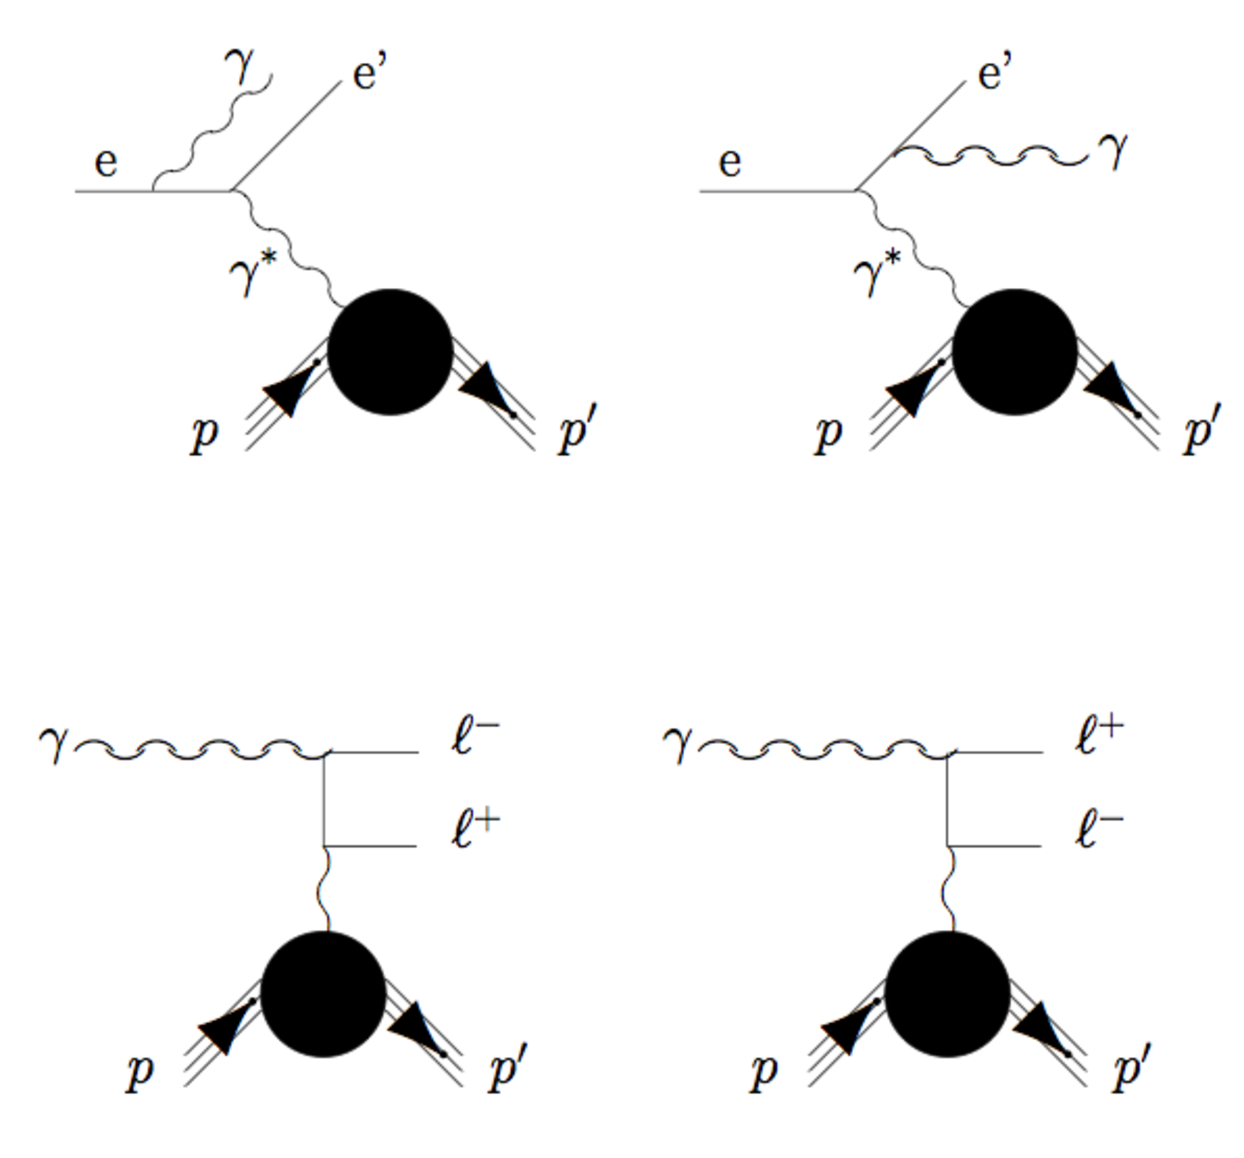
\includegraphics[width=0.8\textwidth]{allbh.pdf}
\end{center}
\caption{Top: the BH diagrams for DVCS. Bottom: the BH diagrams for TCS.
In DDVCS, all four contributions are present (the DVCS-BH diagrams have to
be ``completed" by the decay into a lepton pair of the final state photon 
and in the TCS-BH diagrams, the initial state real photon must
emerge from an electron beam).}
\label{fig:allbh}
\end{figure}

While no experimental data have been published related to TCS (and DDVCS), quite
some data has already been released related to DVCS (on the proton). 
Limiting ourselves to the valence (JLab) region, unpolarized cross 
sections~\cite{carlos,Jo:2015ema}, beam spin asymmetries~\cite{fx} and 
longitudinally polarized target spin asymmetries~\cite{shifeng,erin,Pisano:2015iqa}
(as well as double spin beam-target asymmetries) have been measured. 

These past few years, several groups~\cite{fitmuller,herve,fitmick,fithermes,fittsa,fitall} 
have developped fitting codes and algorithms aimed at extracting the GPD information 
from these DVCS data. We recall the complexity of the task due to,
in particular, the BH contribution in addition to DVCS. These fitting algorithms have 
nevertheless succeeded in extracting
the quantities $H(\pm\xi,\xi,t)$ and $\tilde{H(\pm\xi,\xi,t)}$ at the $\approx 30$\% level
for different values of $\xi$ and $t$ (see Ref.~\cite{rpp} for a compilation of the
fit results). Although the  information thus obtained is already very valuable 
and provides first constraints on GPD models, it is very desirable to extract
the quantities where the first two arguments of the GPDs, $x$ and $\xi$,
are decoupled (i.e. $x\neq\xi$). For instance, ``nucleon imaging"
requires the knowledge of $H(\xi,0,t)$ (and ` for the
other GPDs). With results from DVCS (and TCS) alone, this is not possible.

The way to avoid the $x$-integration issue is DDVCS. Compared to DVCS,
DDVCS contains an additional kinematic lever arm with the timelike virtuality of the
final photon which can can now be varied (by measuring the invariant mass of the
decay leptons pair).
Fig.~\ref{fig:diags} illustrates this where the {\it plus}-components 
(in light-cone kinematics) of
the longitudinal momentum fraction of the quarks and photons are
indicated. In the DDVCS case, the kinematics of the 2 photons 
(incoming and outgoing) is described by 2 variables, $\xi$ and 
$\xi^\prime$, which can be independently varied (whereas, in DVCS,
only $\xi$ can be varied). For DDVCs, there are two diagrams
(only the ``direct" one is shown in Fig.~\ref{fig:diags}) and
their propagators read:

\begin{equation}
{1 \over {x - (2\xi^\prime-\xi) + i \epsilon}} + 
{1 \over {x + (2\xi^\prime-\xi) - i \epsilon}}
\label{eq:ddvcs}
\end{equation}

Therefore, the DDVCS amplitude is proportional to: 
\begin{equation}
\int_{-1}^{+1}d x {{H(x,\xi,t)} \over {x - (2\xi^\prime-\xi) + i \epsilon}}+...
\label{eq:ddvcs2}
\end{equation}

Then, by measuring an observable proportional to the imaginary part of the 
DDVCS amplitude (for instance, the beam asymmetry, like in the DVCS case),
one has access, in a concise notation, to $H(2\xi^\prime-\xi,\xi,t)
+H(-(2\xi^\prime-\xi),\xi,t)$ (keeping the contribution of the crossed term
of Eq.~\ref{eq:ddvcs}.
We refer the reader to Refs.~\cite{Guidal:2002kt,ddvcs_bm1,ddvcs_bm2} 
for the details of the formalism. This therefore allows for maping the GPD's along each
of the three axis ($x$, $\xi$ and $t$) as the three variables can now 
be varied independently. 

Experimentally, $\xi^\prime=\frac{x_B}{2-x_B}$,
i.e. it is fully defined by the detection of the scattered electron,
and $\xi=\xi^\prime\frac{Q^2+Q'^2}{Q^2}$, i.e. it requires 
in addition the determination of the (squared) invariant mass of the lepton
pair $Q'^2$. In other words, if one fixes $x_B$, one defines uniquely $\xi^\prime$
and if one fixes $Q^2$ and $Q'^2$ according to the combination in the
previous sentence, one defines uniquely $\xi$. In order
to access the combination $H(2\xi^\prime-\xi,\xi,t)+H(-(2\xi^\prime-\xi),\xi,t)$,
one should thus aim at measuring the DDVCS beam asymmetry at fixed $x_B$,
$Q^2$ and $t$ for a series of $Q'^2$ values (one can actually also vary $Q^2$,
as long as the combination $\frac{Q^2+Q'^2}{Q^2}$ remains constant
so as to keep $2\xi^\prime-\xi$ fixed).

Fig.~\ref{fig:asym_ddvcs} shows for instance the predicted beam spin asymmetries
for the DDVCS process at typical JLab beam energies for different $Q'^2$
values. We recall that this asymmetry arises
from the interference between the DDVCS and the associated Bethe-Heitler 
processes, which are a generalization of the four diagrams of Fig.~\ref{fig:allbh} 
(the final state real photon of the ``DVCS-BH" diagrams is to decay
into a lepton pair and the initial state real photon of the ``TCS-BH" diagrams
is to be radiated from an electron beam). One recognizes the familiar
sinus-like shapes as a function of $\phi$, the azimutal angle
between the leptonic and hadronic planes.
We also recall that only $Q'^2=0$ can be accessed in DVCS.
The dependence on $Q'^2$ reflects the variation of the first argument
of the GPD ($x=2\xi^\prime-\xi$) for a given second argument $\xi$ (i.e. $x_B$).
Fig.~\ref{fig:asym_ddvcs} shows that there is a strong sensitivity 
which should ultimately allow the extraction of the GPDs in the $(x,\xi)$ plane.

\begin{figure}[htbp]
\begin{center} 
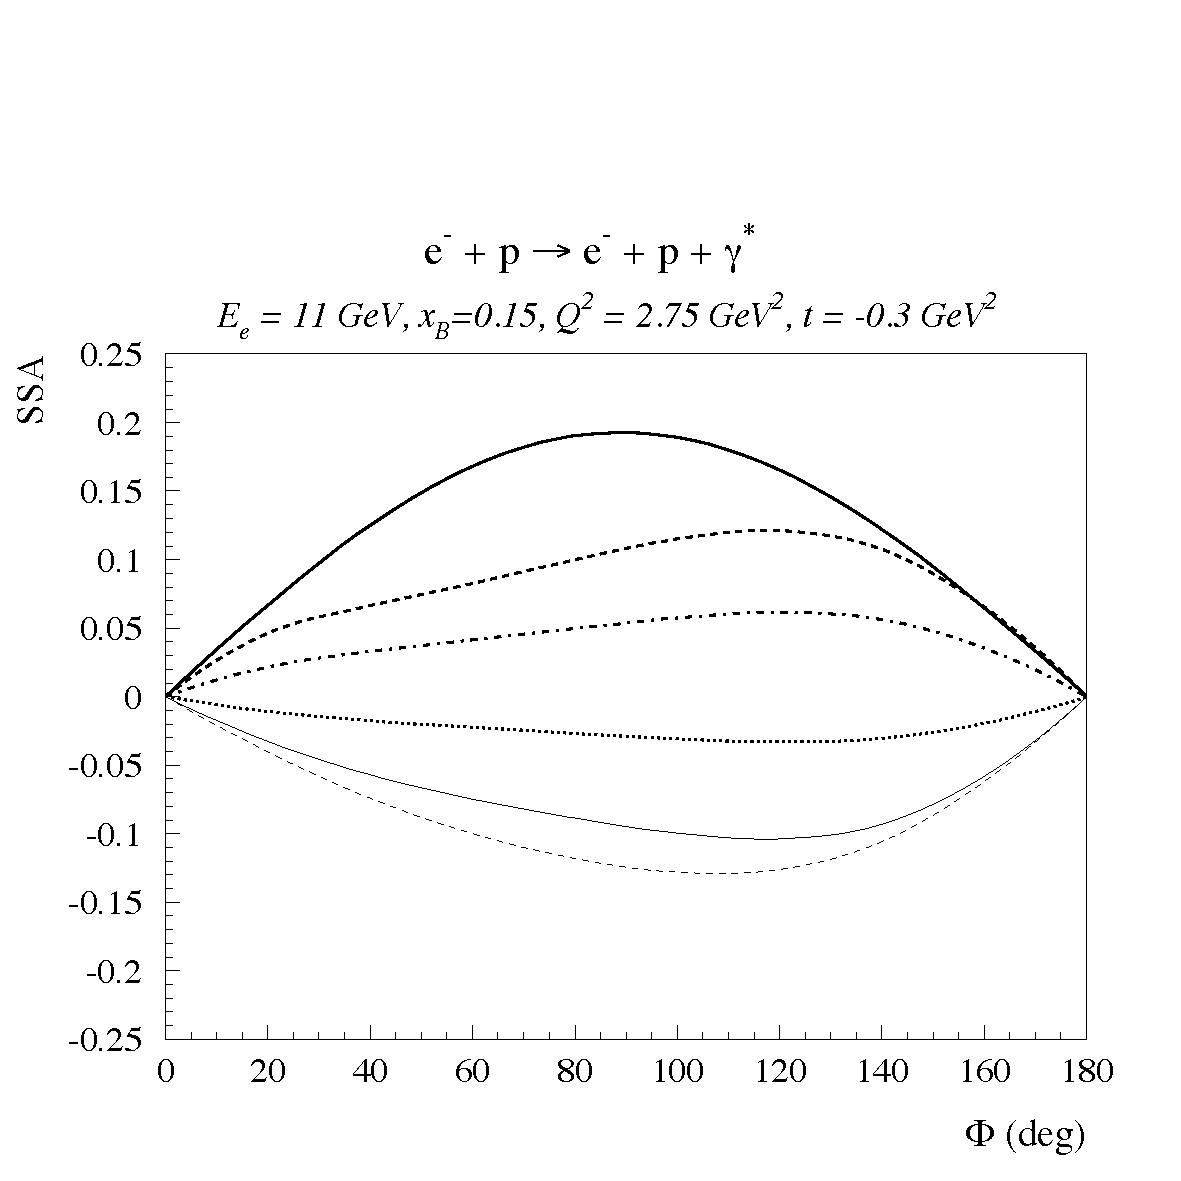
\includegraphics[width=1\textwidth]{asymm_ddvcs.pdf}
\caption{Beam spin asymmetry for the reaction $ep\to e^\prime p\mu^+\mu^-$ (DDVCS+BH) 
for different virtualities of the lepton pair~:
$Q'^2$ = 0. (thick solid line), 1.5 (thick dashed line), 2. (thick dash-dotted line), 2.8 (dotted line)
3.6 (thin solid line) and 4.4 GeV$^2$ (thin dashed line). Calculations and predictions 
from~\cite{Guidal:2002kt}. The kinematics has been integrated over the
2 decay angles.}
\label{fig:asym_ddvcs}
\end{center}
\end{figure}

In Fig.~\ref{fig:asym_ddvcs}, it is very interesting to note the change
in sign of the beam spin asymmetry as one goes from the region $Q'^2<Q^2$
to the region $Q'^2>Q^2$. it can be said that one goes from the
``spacelike-dominated" region to the ``timelike-dominated" region,
or from the ``DVCS-dominated" region to the ``TCS-dominated" region.
It was shown in Ref.~\cite{Muller:2012yq} that the TCS amplitude is the conjugate
of the DVCS amplitude. One can therefore understand the change in
sign of the beam spin asymmetry in Fig.~\ref{fig:asym_ddvcs} as one crosses 
the $Q^2=Q'^2$ region as a change in sign of the imaginary
part of the DDVCS amplitude. This is a prediction of the ``handbag"
formalism and a very strong test that one is in the right regime
to access GPDs. One should note that the region around $Q'^2=Q^2$
might not directly applicable to the GPD formalism. Indeed, in this
region, the quark in the propagator of the DDVCS diagram in Fig.~\ref{fig:diags}
has a momentum close to 0 as $Q'^2=Q^2$ is essentially equivalent
to $2\xi^\prime-\xi=0$. Therefore, pQCD factorization will break down
and soft scales and mechanisms will enter into play. Even though this
particular region $Q'^2=Q^2$ might not be directly interpretable
in terms of GPDs, it should clearly be extremely interesting to
make measurements at those kinematics to understand the transition
between soft and hard mechanisms.

\begin{figure}[htbp]
\begin{center} 
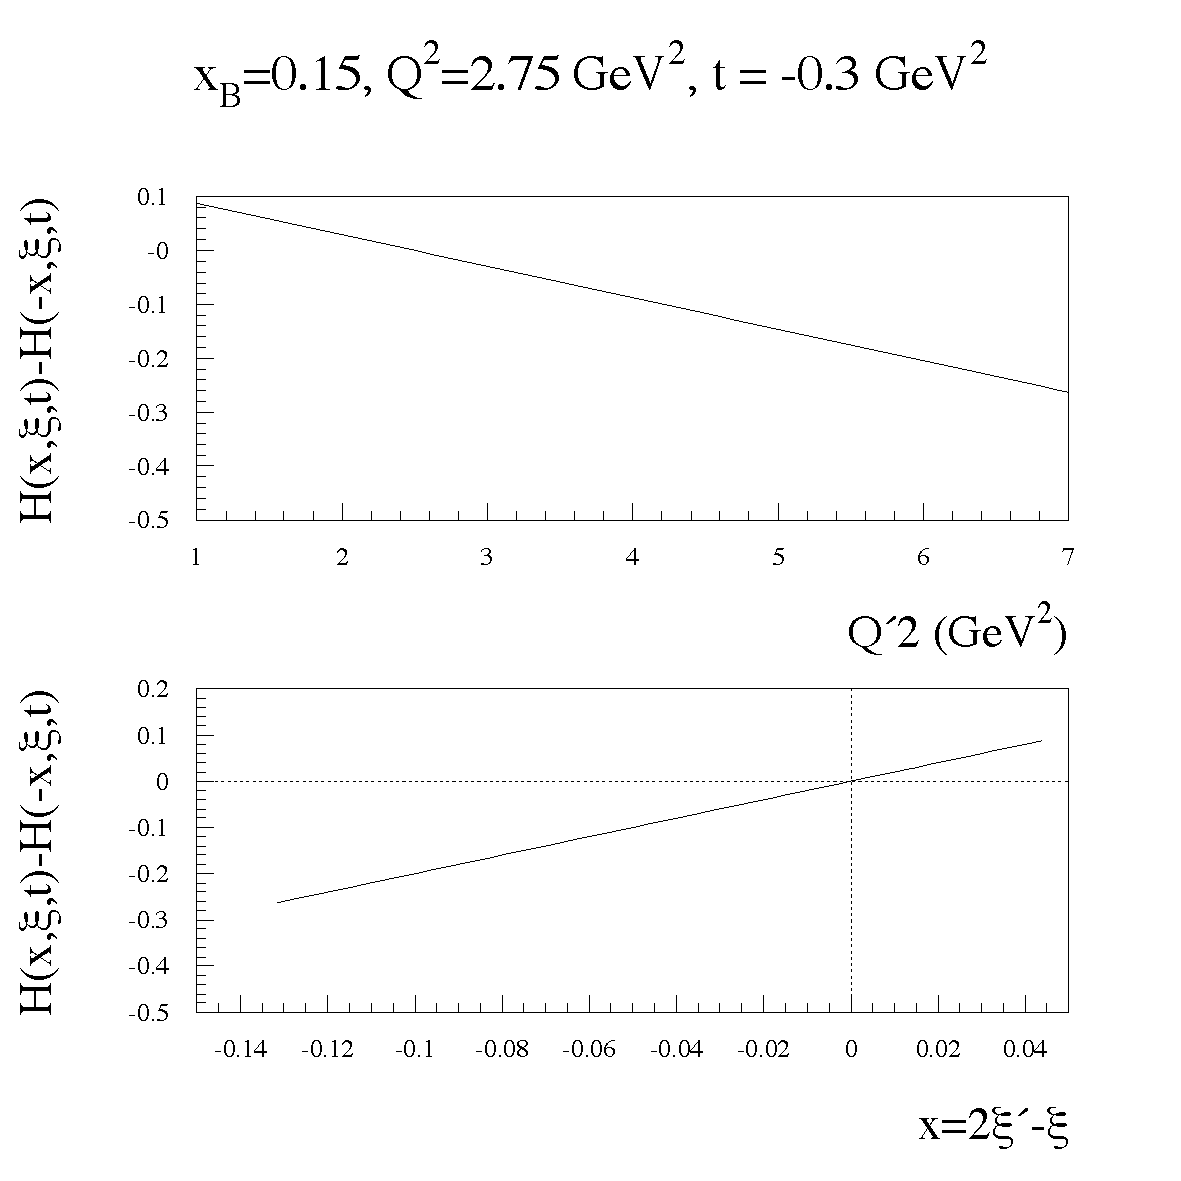
\includegraphics[width=1\textwidth]{scan_ddvcs.pdf}
\caption[]{Assuming the dominance of the $H$ GPD in the DDVCS beam spin asymmetry,
the GPD combination $H(2\xi^\prime-\xi,\xi,t)+H(-(2\xi^\prime-\xi),\xi,t)$
that can be accessed, as a function of $Q'^2$ (top panel)
or equivalently $2\xi^\prime-\xi$ (bottom panel), for fixed $\xi^\prime$ (i.e.
$x_B$) and fixed $t$. In the bottom panel, the negative $2\xi^\prime-\xi$
region allows to access the $-(H(2\xi^\prime-\xi,\xi,t)+H(-(2\xi^\prime-\xi),\xi,t))$
GPD combination for positive $2\xi^\prime-\xi$, due to the symmetry of the
problem.}
\label{scan-ddvcs}
\end{center}
\end{figure}

In Fig.~\ref{scan-ddvcs}, we show the range in $2\xi^\prime-\xi$
that can be accessed at the particular kinematics: $E_e$=11 GeV,
$x_B$=0.15 (i.e. $\xi\approx$0.8), $Q^2$=2.75 GeV$^2$ and $-t$=0.3 GeV$^2$,
by varyong $Q^2$ from 1 to 7 GeV$^2$. One notes in particular
the (anti-)symmetry around $2\xi^\prime-\xi$ which reflects the
quasi (anti-)symmetric behavior of the beam spin asymmetry of
Fig.~\ref{asym-ddvcs} around $Q^2=Q'^2$. One has therefore
two relatievly independent ways of measuring the same
combination of GPDs $H(2\xi^\prime-\xi,\xi,t)+H(-(2\xi^\prime-\xi),\xi,t)$:
in the region $Q^2<Q'^2$ and in the region $Q^2>Q'^2$. Only the sign
of the combination varies as one amplitude is the conjugate of the other.

Of course, the downside of the DDVCS process is however the very low cross section
involved. Indeed, due mainly to the extra $\alpha_e\approx 1/137$ coupling
introduced by the decay of the outgoing photon into the lepton pair,
the cross section is about a factor 300~\cite{Guidal:2002kt} less than the
DVCS process, at $Q'^2\approx .3$ GeV$^2$ for instance. 

We recall that the beam spin asymmetry for DVCS has been measured~\cite{fx}
for $\approx$ 20 ($x_B$, $Q^2$, $t$) bins with the JLab 6 GeV beam 
and the CLAS detector with a luminosity of 10$^{34}$cm$^{-2}$s$^{-1}$.
As we will be shown in the following of this document, it is anticipated
to run with the JLab 12 GeV beam and the CLAS12 detector at a luminosity
of 10$^{37}$cm$^{-2}$s$^{-1}$. Intuitively, it can therefore be anticipated
that the DDVCS beam spin asymmetry measurement should be feasible,
taking also into account an extra factor for the final state lepton pair
detection efficiency.

%\end{document}
